\section{Evaluation}
\subsection{Prüfung der Anforderungen}

Dieser Abschnitt behandelt in wie weit das beschriebene Konzept die in Anschnitt \ref{anforderungen} aufgelisteten Anforderungen erfüllt. Die jeweilige Anforderung wird zunächst wiederholt und anschließend genauer untersucht.

\subsubsection{1) Transparente Einzahlungen}
\textit{Die Einzahlung jedes Endnutzers ist für jeden anderen Endnutzer nachprüfbar.}\\\\
Einzahlungen geschehen genau wie bei Bitcoin innerhalb von Transaktionen, die in die Blockchain geschrieben werden. Diese Anforderung ist also auch im Falle von Ethereum erfüllt.
\subsubsection{2) Gewinnerauswahl durch Zufallsfaktor}
\textit{Die Auswahl des Gewinners ist von einem zufälligen Faktor abhängig, auf den weder die Anwendung noch die Endnutzer einen Einfluss haben.}\\\\
Genau wie bei Bitcoin findet die Gewinnerauswahl basierend auf einem aus dem Proof-of-Work Blockhash statt. Die in Kapitel \ref{btc_evaluation} betrachtete Analyse gilt somit genau so für Ethereum außer, dass der Mining Reward 3 Ether beträgt und durchschnittlich alle 12 Sekunden ausgeschüttet wird. In Zukunft plant Ethereum von einem Proof-of-Work Algorithmus auf einen Proof-of-Stake Algorithmus umzusteigen. Proof-of-Stake und die daraus resultierenden Auswirkungen werden in Kapitel \ref{pos} betrachtet.
\subsubsection{3) Nachprüfbarkeit des Zufallsfaktor}
\textit{Jeder Endnutzer kann die Echtheit des zufälligen Faktors eigenständig nachprüfen.}\\\\
Der zur Gewinnerauswahl verwendete Blockhash ist zum Zeitpunkt der Auszahlung bereits in der öffentlichen Blockchain verankert und kann somit überprüft werden.
\subsubsection{4) Transparente Auszahlungen}
\textit{Die Auszahlung an den Gewinner muss transparent und somit für jeden Endnutzer nachprüfbar sein.}\\\\
Die Auszahlung wird durch die vom Nutzer initiierte \code{payout} Transaktion ausgelöst und vom Smart Contract vorgenommen. Das Verfahren der Auszahlung ist durch den unveränderlichen Smart Contract Code in Stein gemeißelt. Die Konsensregeln und die dahinter liegende Spieltheorie garantieren, dass dieser auch genau so ausgeführt wird. Obwohl die \code{payout} Transaktion nicht direkt Geld auf die Auszahlungsadresse des Gewinners überweist, kann der Endnutzer dennoch sicher sein, dass eine Auszahlung stattgefunden hat, wenn die \code{payout} Transaktion wie in Abbildung \ref{fig:contract_payout_txn} im Status \code{success} vorliegt.
\subsubsection{5) Fairheit des Spiels}
\textit{Jeder Endnutzer besitzt die gleiche Gewinnwahrscheinlichkeit und niemand wird benachteiligt.}\\\\
Damit keiner der Spieler einen Vorteil hat, muss jeder Topf-Platz die gleiche Gewinnwahrscheinlichkeit haben.
Dies ist gegeben, falls jeder Teilnehmer a) die gleiche Anzahl Gewinnzahlen zugeordnet bekommt und b) falls die möglichen Blockhash-Werte für die Gewinnerauswahl gleichverteilt sind.

a) Statt wie bei Bitcoin ausschließlich die letzte Ziffer des Blockhashs für die Gewinnerauswahl zu verwenden und als Konsequenz lediglich Töpfe der Größe 2, 5 und 10 anzubieten, wird bei Ethereum der gesamte Blockhash zur Gewinnerauswahl verwendet. Dies führt zu beliebig großen Töpfen, bei denen einige Teilnehmer genau eine Gewinnzahl mehr haben können. Da jeder Spieler in der Praxis mehrere Millionen von Gewinnzahlen hat, kann man diesen theoretischen Vorteil vernachlässigen.

b) Abschnitt \ref{eth_distribution} zeigt, dass die von Ethereum eingesetzte \code{Keccak-256} Hashfunktion gleichverteilte Werte liefert.


\subsection{Aufruf der Auszahlungstransaktion}
Wie bereits in Abschnitt \ref{eth_konzept} betrachtet, ist der Aufruf deiner Funktion zur Auszahlung unumgänglich. Da der Smart Contract dies nicht selber kann, muss der Aufruf entweder von außerhalb oder von einem Anderen Smart Contract kommen.

a) Aufruf von außerhalb:\\
Der Aufruf kann wie in der Implementierung vom Gewinner ausgeführt werden. In diesem Fall zahlt der Gewinner die Transaktionsgebühr und erhält den gesamten Topf-Betrag. Der Gewinner ist dafür zuständig die Funktion rechtzeitig aufzurufen, da der Gewinn sonst in den nächsten Topf übergeht. Eine andere Möglichkeit ist es, dass die Glücksspielanwendung den Smart Contract überwacht und die \textit{payout} Funktion rechtzeitig aufruft. In diesem Fall müsste die Transaktionsgebühr von der Glücksspielanwendung gezahlt werden oder Funktionalität in den Smart Contract eingebaut werden, die die Transaktionskosten vom Topf-Betrag abzieht und der Glücksspielanwendung zurückerstattet. Allerdings verlässt sich der Gewinner dann auf die Anwendung und geht dadurch ein Risiko ein.

b) Aufruf durch Smart Contract:\\
Man kann in der Theorie den Ansatz des Ethereum Alarm Clock \footnote{\url{http://www.ethereum-alarm-clock.com/}} Contracts \footnote{\url{https://etherscan.io/address/0x6c8f2a135f6ed072de4503bd7c4999a1a17f824b}} verwenden, um eine gewünschte Smart Contract Funktion zu einem späteren Zeitpunkt auszuführen. Man spezifiziert dazu welche Funktion man wann (in welchem Blockzeitraum) ausführen möchte und zahlt für die anfallenden Transaktionsgebühren im Voraus. Dies erlaubt, dass eine ganze Reihe von Funktionen sich bei dem Alarm Clock Contract registrieren. Wird nun der Alarm Clock Contract von einem durch einen privaten Schlüssel kontrollierten Account ausgelöst, werden alle registrierten Funktionen aufgerufen. Leider liefert diese Vorgehensweise keine  Garantie, da eine registrierte Funktion nur aufgerufen wird, falls der Alarm Clock Contract aufgerufen wird. Die Glücksspielanwendung müsste also einspringen, sobald niemand anderes bereit ist den Alarm Clock Contract anzustoßen. Es handelt sich also lediglich um eine Vorgehensweise um Transaktionsgebühren mit anderen Ethereum Nutzern zu teilen.

\subsection{Verteilung der Hashfunktion Keccak-256}\label{eth_distribution}

Ethereum verwendet die kryptographische Hashfunktion Keccak-256.
Die folgende Monte-Carlo-Simulation zeigt, dass die Hashwerte der Hashfunktion Keccak-256 gleichverteilt sind.
\begin{verbatim}
h=Keccak-256 n=1000000
for i 1 -> n
    hash = h(i);
    result[uint(hash)%10]++
\end{verbatim}
\begin{minipage}{0.5\textwidth}
\begin{verbatim}
Ausgabe:
result[0] =  99227
result[1] = 100479
result[2] = 100163
result[3] =  99804
result[4] =  99945
result[5] = 100208
result[6] = 100403
result[7] = 100438
result[8] = 100035
result[9] =  99298
\end{verbatim}
\end{minipage}
\begin{minipage}{0.5\textwidth}
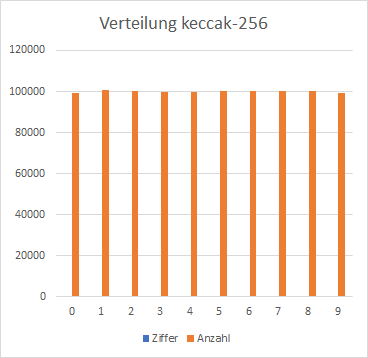
\includegraphics[width=\textwidth]{Figures/verteilung_keccak256}
\centering
\decoRule
\captionof{figure}{Verteilung der Keccak-256 Hashfunktion}
\label{fig:verteilung_keccak256}
\end{minipage}

\subsection{Sicherheit von Smart Contracts}
Bei Smart Contracts handelt es sich um öffentliche, für jeden ausführbare und unveränderliche Software. Beinhaltet diese einen Software Fehler, ist dieser ausnutzbar und kann nicht behoben werden. Smart Contracts verwalten in der Regel Geld oder Token, die einen finanziellen Wert repräsentieren. Bei der Entwicklung eines Smart Contracts ist somit oberste Vorsicht geboten. \todo{Hier zuerst: Durch einen kritischen Fehler im the DAO smart Contratct wurden Millionen verloren... dann erst details was the DAO ist.vllt als fussnote} Das Beispiel von the DAO zeigt, zu welchen katastrophalen Folgen Sicherheitslücken in Smart Contracts führen können.
Bei the DAO handelt es sich um einen von Christoph Jentzsch programmierten und am 20ten April 2016 auf der Ethereum Blockchain veröffentlicht Smart Contract\footnote{\url{https://etherscan.io/address/0xbb9bc244d798123fde783fcc1c72d3bb8c189413\#code}}.
The DAO ist ein Kapitalfond, der es sich zur Aufgabe gemacht hat in Blockchain Technologie zu investieren. Bei dem initialen 28zig tägigen Crowdsale wurden mehr als 150 Millionen Dollar von über 11 Tausend Investoren eingesammelt. Investoren haben Kapital in Form von Ether eingezahlt und als Gegenleistung eine entsprechende Anzahl Token als eine Art Stimmrecht erhalten. Investitionsentscheidungen dieser \textbf{d}ezentralen \textbf{a}utonomen \textbf{O}rganisation werden mithilfe des Smart Contracts durch einen dezentral erarbeiteten Konsens getroffen. Durch das Ausnutzen eines nicht trivialen Fehlers im Smart Contract Code schaffte es ein Hacker einen großen Teil des Kapitals an eine von ihm kontrollierte Adresse auszuzahlen. Eine genaue Beschreibung des Angriffes findet man unter \cite{eth_dao_hack}.

Die Solidity Dokumentation \footnote{\url{https://solidity.readthedocs.io/en/develop/security-considerations.html}} listet eine Reihe von Beispielen, die die Sicherheit von Smart Contracts betreffen. Entwickler sollten sich dieser bewusst sein, bevor sie einen Smart Contract veröffentlichen der Geld verwaltet.
\todo{Sicherheitsaspekt auf eigenen Smart Contract beziehen.}

\if
Hier dann noch darauf eingehen, dass man auf keinen Fall bock.timestamp verwenden sollte, da Miner auf diesen einen direkten Zugriff haben können.

https://ethereum.stackexchange.com/questions/19341/address-send-vs-address-transfer-best-practice-usage

Hier dann nur darauf eingehen, dass falls man die Auszahlung mittels der unsicheren Methode macht ein BUG besteht. 

Anscheinend ist bei address.transfer aber sicher, dass kein contract code ausgeführt wird. Es gibt allerdings 3 Möglichkeiten zu senden.
Eine ist unsicher.

\begin{lstlisting}[basicstyle=\small]
function payout() public{
    assert(potClosed);
    assert(block.number>payoutBlockNumber);
    potClosed = false; //fixes bug
    payoutBlockHash = block.blockhash(payoutBlockNumber); 
    if(payoutBlockHash == 0){
        nbrOfMissedPayouts++;
    }else{
        winner = uint(payoutBlockHash) % NBR_OF_SLOTS;
        address winnerAddress = payoutAddresses[winner];
        uint amount= EXPECTED_POT_AMOUNT*NBR_OF_SLOTS;
        amount += EXPECTED_POT_AMOUNT*NBR_OF_SLOTS*nbrOfMissedPayouts;
        winnerAddress.transfer(amount); // send pot amount to winner
        nbrOfMissedPayouts = 0;
    }
    nbrOfParticipants=0;
}
\end{lstlisting}


\fi
